%!TEX root = ../thesis.tex
\chapter{Background Information}
% If you like chapter abstracts ...
\dblspace
\begin{quote}{\em %!TEX root = ../thesis.tex
In this chapter we review some central background to the coming chapters. A synopsis of cardiac anatomy is followed by a brief on the electrophysiolical structure and function of the heart on the cellular, tissue and organ scale. First we discuss the overall activation sequence during one full beat of the heart, along with the problems that can arise during this process. We go on to discuss the cellular machinery which transduces this cycle, and how tissue structure mediates its propagation. We explain a commonly implemented continuum-based model of wave propagation known as the bidomain model, and examine how this model can be simulated upon three-dimensional finite element meshes, constructed from morphologies extracted from medical images. We conclude the chapter with an overview of the imaging techniques that are used to reconstruct and align volumes from raw imaging data, and then to extract the tissue features and morphologies from the volumes.}\end{quote}

\section{Cardiac Anatomy}
  The heart is a pump which circulates blood through the lungs and around the body. Throughout a human life, the heart contracts approximately 100,000 times per day, beating around 2.5 billion times in an average 66-year lifetime. The heart is divided into four chambers, two superior atria and two inferior ventricles. Deoxygenated blood from the body flows into the right atrium and into the right ventricle, from where it is pumped through the lungs in order to exchange CO$_2$ with oxygen. Blood returns from the lungs and enters the left atrium and subsequently the left ventricle. Finally, the left ventricle pumps blood back out to the body via the aorta, the widest artery in the body. Retrograde flow through the aorta back into the left ventricle is prevented by the aortic valve.
  
  \begin{figure}[htbp]
    \centering
    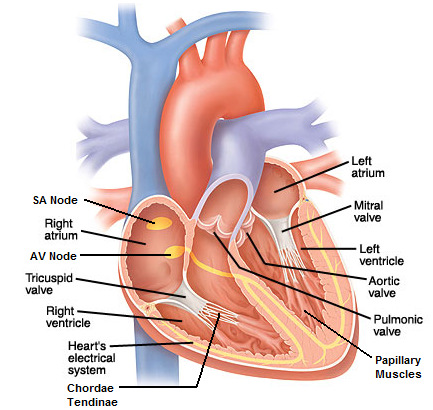
\includegraphics[width=0.6\textwidth]{Ch2/Figs/interior_heart_anatomy}
    \caption{Schematic of the main anatomical features and structures of the heart. Blue vessels carry deoxygenated blood and red vessels oxygenated blood. Note the thicker walls of the left ventricle, to provide enough pressure to force blood around the entire body. The two atrioventricular valves, the tricuspid and the mitral valves, are labelled. From the Ed Dardanell Heart and Vascular Centre (www.forbesheartcenter.com).}
    \label{fig:heart}
  \end{figure}  

The heart walls are comprised mostly of striated muscular tissue known as myocardium. The outer, middle and inner heart walls are termed the epicardium, mid-myocardium and endocardium, respectively. At the cellular level, myocytes are the long oblate myocardial cells, locally aligned with each other. Myocytes are further arranged into discrete myocardial sheets, separated by cleavage planes, as seen in Figure~\ref{fig:sheets}. The myocytes in each sheet will contract in a unified direction and the sheets will slide over each other, maximising the volume output and mechanical efficiency of the heart. A muscular septal wall through the centre of the heart separates oxygenated blood in the right chambers from deoxygenated blood in the left. The eponymous atrioventricular valves prevent blood from leaking back into the atria from the ventricles; these are controlled by the papillary muscles, contractile pillars connected to the valves at their tip and to the endocardium at their base.

  \begin{figure}[htbp]
    \centering
    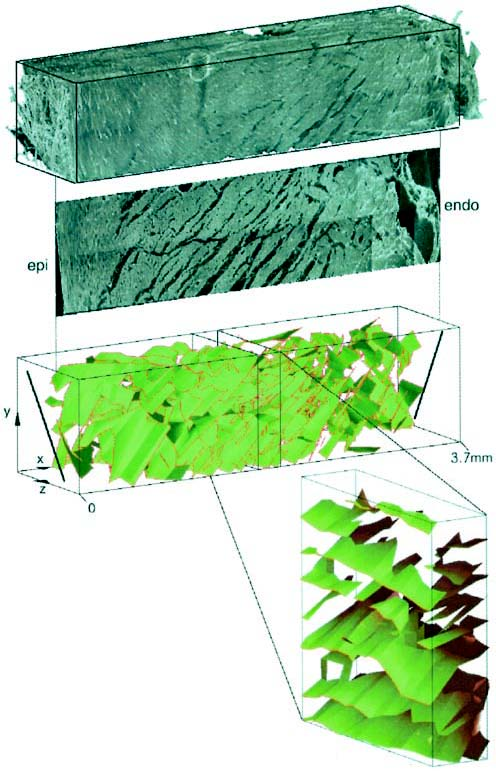
\includegraphics[width=0.6\textwidth]{Ch2/Figs/sheets}
    \caption{The top cuboid is a small volume of rat left ventricular myocardium from \cite{Hooks2002}, reconstructed from a series of 2-D multiple histological images. Just below, a transmural slice from the reconstructed volume shows a complex network of cleavage planes that course between layers of myocytes. Each layer is of around 80$\mu$m thick. The extracted cleavage planes are shown below in green, through the entire rat tissue block and a smaller midwall subsection. Myofiber orientation is shown on the epicardial and endocardial surfaces.}
    \label{fig:sheets}
  \end{figure}

  The vascular system is divided at the heart into two subsystems: the pulmonary vascular system, which transports blood from the right ventricle, through the lungs, and back to the left atrium; and the systemic vascular system, which carries blood from the left ventricle, around the rest of the body, and back to the right atrium. Part of the systemic system is the coronary vascular system, supplying the heart tissue with oxygen and nutrients and removing waste. The main arteries supplying the myocardium stem from the root of the aorta, immediately above the aortic valve, and run along the outer surface of the heart; they are thus named the epicardial coronary arteries. The positioning of the coronary arteries on the surface, away from the high systolic pressures of the endocardium, allow them to remain turgid and autoregulate to supply the heart tissue with appropriate blood flow.

\section{Cardiac Electrophysiology}
\label{sec:electrophysiology}
  \subsection{Activation Sequence}
  \label{sub:activation_sequence}
    Contraction of the heart is controlled by a complex sequence of electrical activation. The sino-atrial node or pacemaker, positioned at the top of the right atrium (see Figure~\ref{fig:heart}), is a cluster of self-excitable myocytes that depolarises at a regular interval, dictating the rate of heart pumping. From there a depolarising wave quickly spreads across the right and left atria, so that they contract in unison and force blood into the ventricles. An electrical barrier isolates the atria from the rest of the heart, and the atrioventricular node provides the only pathway to the ventricles. It delays the signal to allow the atria to contract fully, before stimulating the Purkinje fibres via the bundle of His. The Purkinje fibres are long transduction cells sheathed in an insulating layer of fat, much like neurons. They comprise a network that runs from the bundle of His along the endocardium and through the ventricular cavities, dividing dentritically across both ventricles to carry the electrical signal throughout the ventricular walls. From here, the action potential spreads through the myocardium from endo-~to epicardium, effecting a synchronised contraction of the ventricles and pumping blood to the lungs and body.
    
    Pathological deviations from this highly coordinated electromechanical process severely debilitate cardiac output. Arrhythmia occurs when a reentrant spiral wave manifests within the myocardium, overriding the natural contraction sequence controlled by the sino-atrial node. At the centre of the reentrant wave is a phase singularity, a small area of ambiguous activation that acts as the organising node of the arrythmia. These more organised arrhythmias can degenerate further into more complex arrhythmic episodes termed fibrillation, as the reentrant wave breaks up into smaller, more chaotic fragments. Cardiac output during fibrillation is close to zero as asynchronous fluttering ensues, and the condition is fatal within a few minutes. By far the most common treatment at this stage is defibrillation therapy, where high voltages are applied across the heart via metal plates placed either side of the chest cavity.
    
  \subsection{Myocyte Excitation}
  \label{sub:myocyte_excitation}
    Cardiomyocytes contract as a result of an external electrical stimulus. When at rest, a myocyte has a negative membrane potential, around -90mV. Stimulation above a certain threshold causes depolarisation across the cell membrane, as voltage-gated ion channels are activated and positive ions flood into the cell. The controlled influx and efflux of ions such as Na$^+$, K$^+$, Ca$^{2+}$ and Cl$^-$ through various gates, pumps and exchangers eventually ensures the repolarisation of the cell. The form of the transmembrane potential spanning one complete depolarisation/repolarisation cycle is known as an action potential. Once a cell has been depolarised and has repolarised, for a short period it is immune to further depolarisation. This interval is known as the refractory period. In this way, a maximum action potential frequency is enforced. Ionic connections between adjacent cells called gap junctions ensure a fast and robust propagation mechanism by boulstering electrical coupling.
  
  \subsection{Microstructure and Propagation}
  \label{sub:microstructure_and_propagation}
    As activated myocytes and other electrically active cells stimulate their neighbours, the action potential propagates through cardiac tissue. The frontier of this propagation is known as the wavefront, and the behaviour of this wavefront over time is known as its wavefront dynamics. Cardiac microstructure plays a central role in controlling the speed and direction of cellular activation. Intracellular conduction is quicker than intercellular conduction, and the long, cylindrical shape of myocytes permits faster wave propagation along their fibre direction than perpendicular to it. The cleavage planes shown in Figure~\ref{fig:sheets} that pervade the myocardium act as a conductive barrier, forcing the wave to propagate around them, and thus reducing the overall conduction velocity perpendicular to them when observed on a macroscopic tissue scale. Other insulating artefacts, such as blood vessels, have similar retarding effects. Indeed, they may also serve as arrhythmic anchors, providing an insulated circuit around which phase singularities may oscillate without annihilating themselves.
    
\section{Electrophysiological Modelling}
\label{sec:electrophysiological_modelling}
  \subsection{Cellular and Tissue Modelling}
  \label{sub:cellular_and_tissue_modelling}
    In creating realistic and powerful cardiac models, it is necessary to represent faithfully the electrophysiological processes of the heart at both the cellular and the tissue level. The bidomain model attempts to unify these two scales, by representing the extra-~and intracellular spaces in cardiac tissue as two continua, such that two electrical potential fields $\phi_\text{e}$ and $\phi_\text{i}$ are defined across the tissue space. The transmembrane potential difference is then given by
  
    \begin{equation}
      v = \phi_\text{i} - \phi_\text{e}.
    \end{equation}
  
    The bidomain equations are a pair of coupled differential equations that are based on a reaction-diffusion model of ion flux. They result from imposing conservation of ions and charge throughout the domain. They can be expressed as
  
    \begin{align}
      \beta \left( C_\text{m}\frac{\partial v}{\partial t} + I_\text{ion}\left( \boldsymbol\eta, v \right) \right) - \nabla \cdot \left( \sigma_\text{i} \nabla \phi_\text{i} \right) &= I_\text{istim}, \\
        \nabla \cdot \left( \sigma_\text{e} \nabla \phi_\text{e} +  \sigma_\text{i} \nabla \phi_\text{i} \right) &= I_\text{estim},
    \end{align} 
  
    where $\beta$ is the membrane surface to volume ratio, $C_\text{m}$ is the specific membrane capacitance, $\sigma_\text{e}$ and $\sigma_\text{i}$ are the extra- and intracellular conductivity tensors, and $I_\text{estim}$ and $I_\text{istim}$ are currents into the two domains due to external stimulus. Cardiac tissue exhibits anisotropic conductivity, transmitting current much more readily along the tubular muscle fibres than across them. Accordingly, the principal eigenvectors of $\sigma_\text{e}$ and $\sigma_\text{i}$ are closely aligned with the local myocardial fibre direction. $I_\text{ion}$ is the ionic current from the extracellular into the intracellular domain. In the simplest passive implementation of the bidomain equations, it would be a term linear in $v$, with the proportionality constant equivalent to the conductance per unit area of the cell membrane. This, however, is highly unrealistic and in practice, $I_\text{ion}$ is a complex function, associated with a non-linear cell electrophysiology model. In this case, $\boldsymbol\eta$ is a vector of the state variables that parameterise the cell model. The cell model dynamics are governed by the set of equations
  
    \begin{equation}
      \frac{\partial \boldsymbol\eta}{\partial t} = \mathbf{f}\left(\boldsymbol\eta, v \right).
    \end{equation}
  
    The monodomain model is a simplification of the bidomain model, based on the assumption that the intra- and extracellular conductivity tensors are linearly dependent i.e. they only differ by a constant scalar factor. The two potentials $\phi_\text{e}$ and $\phi_\text{i}$ are amalgamated, so that only the potential difference $v$ is parameterised. Whilst less accurate, the resulting set of equations often require orders of magnitude less computation. Yet this advantage cannot be exploited for all purposes, since the regime cannot handle conductivity through baths, interstitial spaces and anywhere in the absence of tissue.
    
  \subsection{Anatomical and Structural Modelling}
  \label{sub:anatomical_and_structural_modelling}
    The equations of tissue state are solved upon volumetric finite element meshes, either of tissue segments, of such organ components as ventricles and atria, or of entire organs. Tissue type geometry is either constructed a priori as a simplistic block, or is extracted from 3D imaging data from MRI or histology. Anisotropic conductivity based on fibre direction is usually incorporated throughout the entirity of the mesh, generated either from a simple mathematical rule, or extracted from histological or diffusion tensor MRI images using image processing algorithms. Fine anatomical detail is rarely included in these models, mainly because it is difficult to obtain.
    
    In summary, the efficient and rigorous solution of electrophysiological wave propagation over a realistic 3-D geometry is a highly complex task, and remains the ongoing effort of many teams of experts in the field. Detailed knowledge of several fields is necessary, including numerics, algorithms, parallel computing and software design practices.

\section{Imaging}
\label{imaging}
  Medical images from a variety of modalities can be used to develop computational meshes that accurately represent cardiac geometry and structure. It is a common problem in medical imaging to match one image to another for the purposes of comparison and validation, or to combine the information gleaned from both. High-resolution MRI images, which can be used to construct relatively detailed geometric meshes, must be aligned with DTMRI data in order to map fibre orientation to the mesh. Randomly oriented histological slices must be aligned either to each other, to an MRI volume or to a coherent set of block face images in order to reconstruct cellular-resolution colour tissue volumes. This process of image alignment is called registration. Physical regions, objects and features must be identified from raw image data, so that meshes may be constructed that reflect the form of the imaged organ. For example, each pixel of the hippocampus of a brain or the vessels in a heart must be labelled for their inclusion in a model. The automation of this identification is known as segmentation. The Insight Toolkit \cite{Yoo2002}, or ITK, is an open-source software toolkit written in C++, used primarily for performing registration and segmentation.
  
  \subsection{Registration} % (fold)
  \label{sub:registration}
    ITK provides a high-level registration framework into which a large selection of functional modules can be swapped, enabling the developer to tailor the registration pipeline to the requirements of the data. The framework consists of the two images to be coregistered, and four main components: a transform, an interpolator, a fitness metric and an optimiser.

    If we consider an image as a function of an n-dimensional point in space, one of the images is designated as fixed, while the other is marked as moving. The transform maps grid points in the fixed image to the equivalent point in the moving image. In general, the mapped points will not fall exactly on grid points in the moving image, and so the interpolator generates a value based on the nearby grid points. Once this is completed, the metric compares the fixed image to the resampled moving image and provides a measure of their similarity, along with other information including the gradient of the similarity measure in the parameter space of the transform. Finally, the optimiser uses the information provided by the metric to decide upon a new transform, in an attempt to generate a better similarity value and thus marry the two images more closely. This iterative process is repeated until a minimum threshold for improvement is reached and final parameters are settled on. Figure~\ref{fig:framework} gives a diagrammatic overview of the relationship between the components of the registration framework.

    \begin{figure}[htbp]
      \centering
      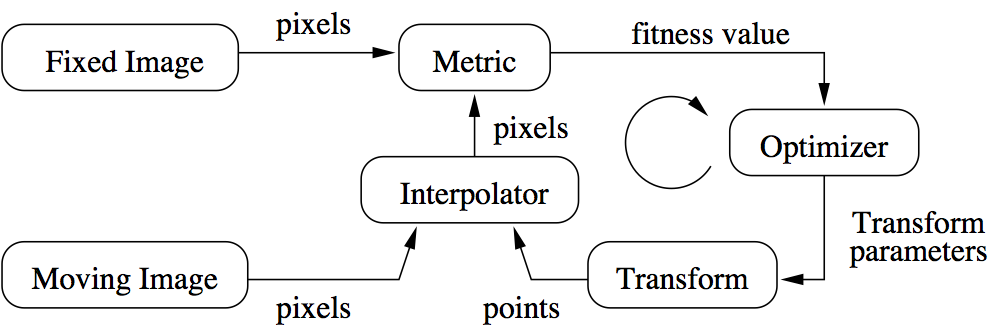
\includegraphics[width=0.85\textwidth]{Ch2/Figs/framework}
      \caption{A schematic of the ITK registration framework. An initial transform is applied to the grid points of the fixed image and an interpolator provides values for each pixel, based on the moving image. The original fixed image and the resampled moving image are then compared by the metric, almost always in a pixelwise fashion, to provide a single-valued measure of fit, and a gradient of this measure with respect to each parameter defining the transform. The optimiser then chooses new transform parameters in an effort to improve the fitness value. The process iterates to convergence.}
      \label{fig:framework}
    \end{figure}
    
    \subsubsection{Transforms} % (fold)
    \label{ssub:transforms}
      ITK provides a comprehensive suite of linear and non-linear transforms. Amongst the linear transforms, there is provided a set of `centered' transforms: rigid, similarity and affine, where the transformation is described in terms of a matrix transformation about an arbitrary centre, followed by a translation, and the centre of rotation is exposed to the optimiser. This leads to a degenerate set of transform parameters leading to the same transformation, but can facilitate a smoother path to minimisation through parameter space. Several non-linear transform classes are also provided, including cubic b-spline and PDEs, all of which may be initialised by a linear bulk transform.
    % subsubsection transforms (end)
    
    \subsubsection{Interpolation} % (fold)
    \label{ssub:interpolation}
      ITK provides four methods of interpolation: nearest neighbour, linear, B-spline and windowed sinc. Nearest neighbour interpolation simply returns the value of the closest pixel in the image being sampled. This requires the least amount of computation of the four methods, but results in a more jagged optimisation function, which could increase the time to convergence, the exact value converged upon, or in rare cases could prevent convergence to the global minimum. More accurately, but slightly more expensively, the value can be linearly interpolated from the four corners of the containing square or eight of the containing cube. Even more accurately, the image intensity can be calculated using B-spline basis functions. However, values may lie outside the range of input image intensities, causing saturation. Finally, the most accurate is the windowed sinc interpolator. Interpolation is based on the Fourier analysis of a sampled smooth spatial function. The pixel intensity is the result of a convolution of the sinc function with a window of neighbouring pixels. This requires by a stretch the most computation. For our purposes, linear interpolation provided the best compromise between efficiency and accuracy.
    % subsubsection interpolation (end)
  
    \subsubsection{Metrics} % (fold)
    \label{ssub:metrics}
      The metrics available in ITK compare the gray-scale intensity of two images to measure how well they are aligned. Masks can be set for both the fixed and moving images to restrict evaluation of the metric within a specified region. The choice of metric critically affects the shape of the optimisation function in the parameter space, and some are only suitable to compare images of the same modality. A mean squares metric requires that equivalent points in the two images are at the same intensity in order to function well. A normalised correlation metric is slightly more flexible in its range of application, but still assumes a linear relationship between equivalent intensities in the two images. A mutual information metric assumes no such relationship. The mutual information between two images is a measure of how much information a random intensity from one image confers about the intensity at the equivalent point in the other image. For example, a region could be uniquely dark grey in one image, but uniquely red in the other. Regardless of the colour or intensity, if a randomly selected pixel turns out to be that exact dark grey in the first image, one can be sure that the same point in the second image is red, and vice versa; mutual information is maximised. If for some reason, these regions were misaligned, that certainty is compromised, and the contribution to the mutual information coefficient from that region is reduced. The mutual information approach is ideally suited to the registration of MRI to histology, where the relationship between intensities is highly complex.
    % subsubsection metrics (end)
  
    \subsubsection{Optimisation} % (fold)
    \label{ssub:optimisation}
    The optimiser iteratively moves through the space defined by the transform parameters from a set of initial coordinates, in an attempt to minimise the cost function evaluated by the metric. ITK provides a range of algorithms to achieve this task in the most efficient and reliable way possible. Throughout the registration process, a gradient descent optimiser was employed. This optimiser is a robust, general purpose algorithm that requires little configuration.
    % subsubsection optimisation (end)
  % subsection registration (end)
  
  \subsection{Segmentation} % (fold)
  \label{sub:segmentation}
    The simplest segmentation algorithm is known as threshold segmentation. Pixels are grouped into two or more segments, based solely on their intensities. The boundaries between the segment intensity ranges are known as thresholds. 
    
    Region growing segmentation algorithms are a class of iterative methods that start from a seed region or set of regions, and evaluate neighbouring pixels in order determine whether to absorb them into the region. When an iteration passes without changing a single pixel of the segmentation, the algorithm is terminated. The exact implementation of region growing algorithms can vary through the criteria for inclusion, the definition of neighbours and the strategy used to visit neighbouring pixels. The connected threshold algorithm includes pixels that fall within a prespecified intensity range, whereas the confidence connected threshold algorithm defines the range dynamically, based on the mean and standard deviation of the current region. 
    
    Level set segmentation is a method to evolve the contour or surface of a region, based not only on the characteristics of the image, but also on the morphology of the region boundary. The image boundary is embedded as the zero level-set in a higher dimensional function called the level-set function $\psi(\mathbf{X}, \mathbf{t})$. $\mathbf{\psi}$ is then evolved via a differential equation:
    
    \begin{equation}
      \frac{d\psi}{dt} = -\alpha\mathbf{A}(\mathbf{x}) \cdot \nabla \psi - \beta P(\mathbf{x})|\nabla\psi| + \gamma\mathbf{Z}(\mathbf{x})\kappa|\nabla\psi|,
    \end{equation}
    
    where the first term moves the level-set according to the vector field \textbf{A}, the second term propagates the level-set normal to its boundary based on an input image $P$, and the third based on the curvature $\kappa$ of the boundary and a spatial modifier image $Z$. A particular level set algorithm might use one or more of these terms, and the scalar constants $\alpha$, $\beta$ and $\gamma$ should be scaled according to the properties of the image and of the initialisation, and the morphology of the underlying object.
    
    The concepts of erosion and dilation are closely tied to that of segmentation, and are in fact implicit in some segmentation implementations. In dilation, a segmentation is expanded to include the neighbours of every pixel within a region. The neighbours are defined by a binary shape function, often circular or square, and of the dimensions of just a few pixels. Erosion is the complementary process, and is equivalent to the dilation of the pixels outside of the region. Morphological opening is the dilation of an erosion of a segmentation. In this way, detailed features of a segmentation such as filaments, edges and regions smaller than the shape function are removed, and the boundary is smoothed. Closing, conversely, is equivalent to a dilation followed by an erosion and, rather than small objects, acts to remove small holes from within the segmented region. Small regions and holes can also be identified by the number of contiguous pixels they are comprised of, and removed without altering the shape of their larger siblings.
    
  % subsection segmentation (end)
% section introduction (end)
